% 2400 signs per page setup:
\documentclass[a4paper, 12pt]{article}

\usepackage{geometry}
\usepackage{amsmath}
\usepackage{color}
\usepackage{graphicx}
\usepackage{array}

% Force images to be where you want with [H]
\usepackage{float}
% images alongside text
\usepackage{wrapfig} 
\usepackage{hyperref}
\usepackage[parfill]{parskip}

% blank pages
\usepackage{afterpage} 

% #http://ctan.org/pkg/{fancyhdr,graphicx,lastpage}
\usepackage{fancyhdr,graphicx,lastpage}

% get the degree symbol
\usepackage{gensymb} 

% subfigures inside of normal figures
\usepackage{subcaption} 

% Glossary / Abbrevations list
\usepackage{glossaries}
\makeglossaries

% Include other files into document
\usepackage{subfiles}

% Appendices
\usepackage{tocloft}
\newlistof{appendices}{apc}{\listappendicesname}
\newcommand{\listappendicesname}{Appendices}
\newcommand{\appendices}[1]{\addcontentsline{apc}{appendices}{#1}}
%\newcommand{\newappendix}[1]{\section*{#1}\appendices{#1}}
\newcommand{\newappendix}[1]{\appendices{#1}}

% Bibliography and refrence manager with Biber
\usepackage[backend=biber, % compile with biber (pdflatex %; biber %; pdflatex %; pdflatex %)
            sorting=none %  none means sort by appearance
            ]{biblatex}
\addbibresource{./sources.bib} % take bibliography resources from this file

% Define margins for page setup
\newgeometry{vmargin={30mm}, hmargin={30mm}, tmargin={30mm}, bmargin={30mm}}

% Shortcut path for graphics
\graphicspath{ {./src/} }

% Header/Footer setup:
\fancypagestyle{plain}{
  \fancyhf{}                                       
  \fancyhead[L]{\center{Surface-EMG Processing \& Classification for Muscle Interfaces}}
  \fancyhead[R]{}
  \fancyfoot[L]{Thomas Alexgaard Jensen \\ University of Southeren Denmark}
  % The \ after thepage makes a spacer..
  \fancyfoot[R]{\thepage\ / \pageref{LastPage}}
}

% Set page style to plain.
\pagestyle{plain} 

% Define Title Page information
\title{\textbf{Surface-EMG Processing \& Classification for Muscle Interfaces}}
\author{Thomas Alexgaard Jensen (tjens18@student.sdu.dk)
\\University of Southeren Denmark
\\
\\Supervisors: 
\\Poramate Manoonpong (poma@mmmi.sdu.dk)
\\Xiaofeng Xiong (xizi@mmmi.sdu.dk)
}
\date{1. June 2023}

% norm symbols for math
\newcommand{\norm}[1]{\lvert #1 \rvert}

% Explanation setup, used for specific words explanation
\newcommand{\explanation}[2]{
\textit{#1: }{#2.}
}


\begin{document}\thispagestyle{empty}
\maketitle
\thispagestyle{empty}
\begin{figure}[h]
\begin{center}
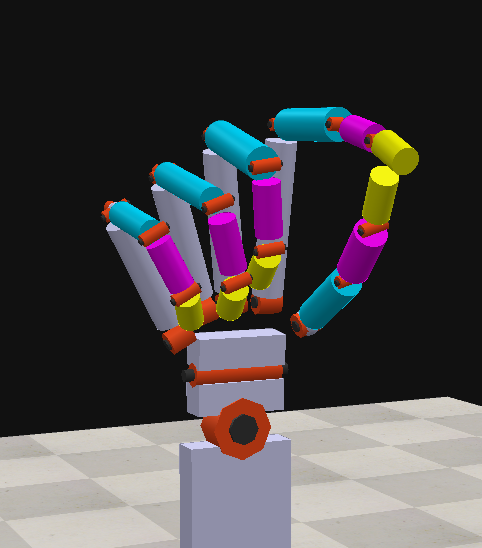
\includegraphics[width=0.8\textwidth]{pulppinch_grip.png}
\end{center}
\end{figure}
%TODO: Picture of setup real hand + sim, in some cool pose


\newpage
\subfile{content/abstract.tex}

% Reset counter to not count front page
%TODO: Do i want to reduce count by 1?
\setcounter{page}{1}

\newpage
\subfile{content/acknowlegdements.tex}
\newpage

\subfile{content/glossary.tex}
\newpage

\tableofcontents
\newpage

\subfile{content/introduction.tex}
\newpage
\subfile{content/problem_specification.tex}
\newpage
\subfile{content/literature_review.tex}
\newpage
\subfile{content/methodology.tex}
\newpage
\subfile{content/test_results.tex}
\newpage
\subfile{content/discussion.tex}
\newpage
\subfile{content/conclusion.tex}
\newpage

\section{Bibliography}
%TODO: Make Figures/tables a indexable countable section
%\section{List of Figures \& Tables}
\listoffigures
\listoftables
%\newpage

\printbibliography
%TODO: Make Refrences a indexable countable section

%TODO: This is not a proper way of having appendices. fix it?
%TODO: Sort into correct order!
\newpage
\listofappendices  % This call Creates a large appendix header
\appendix % This call gets nice A, B, C indexing to appendixes

%\addtocontents{toc}{\cftpagenumbersoff{section}}

The appendices should have been supplied with the report.
Alternatively, see \\
\url{https://github.com/thom9258/masters-thesis/tree/main/report/appendix} \\
for online refrence.

\section{Prosthetic Hand Simulation in CoppeliaSim}
\label{appendix:handsim}

\section{Hand Simulation Poses}
\label{appendix:handsim_poses}

\section{ROS2 Controller for the Prosthetic Hand}
\label{appendix:roscontrol}

\section{Modification \& Replaying Scripts for Motive CSV Files}
\label{appendix:motiveformatting}

\section{Motion-Capture \& sEMG Dataset}
\label{appendix:dataset}

\section{Motive Marker labeling \& Uncleaned marker set}
\label{appendix:motivefixing}

\section{Pre-Processing Filter Graphs}
\label{appendix:preprocessing}

\section{Network Creation/Training/Testing Code}
\label{appendix:networks}

\end{document}
